\documentclass[resume]{subfiles}


\begin{document}
\section{PLL}
\paragraph{CMT} : Clock Management Tile
\paragraph{PLL} : Phase Lock Loop
\paragraph{DCM} : Digital Clock Manager
\paragraph{GCLK} : Global Clock
\paragraph{VCO} : Voltage Controlled Oscillator
\paragraph{DLL} : Delay-locked loop
\paragraph{DFS} : Digital Frequency Synthesis
\paragraph{CDC} : Clock domain crossing
\subsection{Horloges}
2 domaines d'horloge dans le spartan-6
\begin{itemize}
\item 2 horloges I/O jusqu'à \SI{1}{\giga\hertz}, gérées par BUFPLL, 1 pour chaque côté du FPGA
\item 4 horloges I/O jusqu'à \SI{1}{\giga\hertz}, gérées par BUFIO2, 1 pour chaque demi-côté du FPGA
\item max 16 horloges internes jusqu'à \SI{400}{\mega\hertz}
\end{itemize}
1 à 6 CMT (Au maximum 12 DCM et 6 PLL).\\
\begin{figure}[H]
\centering
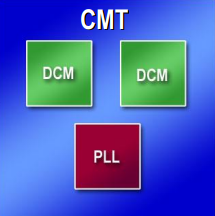
\includegraphics[width=3.00cm]{img_4.png}
\end{figure}
\begin{figure}[H]
\centering
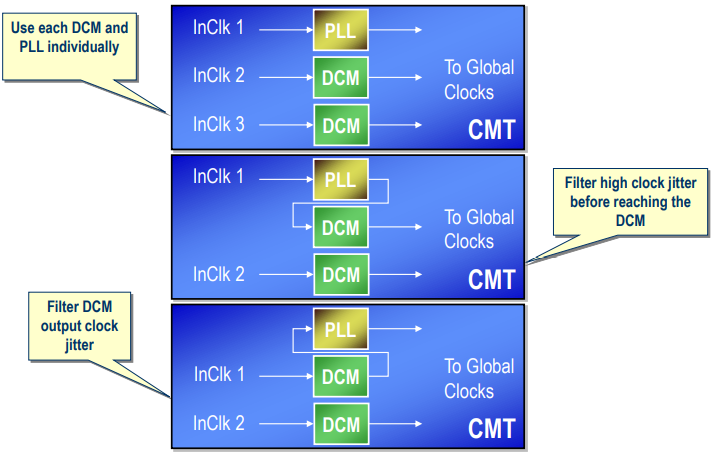
\includegraphics[width=\columnwidth]{img_5.png}
\end{figure}


\subsection{Exemple de génération d'horloge}
\begin{itemize}
\item Utilisation d'une pin GCLK reliée à une horloge précise à \SI{50}{\mega\hertz} (single-ended clock input sur horloge 0 par exemple)
\item Utilisation d'une PLL pour convertir l'horloge 0 en \SI{500}{\mega\hertz} sur l'horloge 1
\end{itemize}
Aussi possible d'utiliser les pins GCLK comme I/O standards si elles ne sont pas utilisées pour les horloges.
\subsection{Réseau d'horloge}
Distribuée en arbre pour avoir un temps de propagation égal à tous les noeuds. Un réseau d'horloge peut aussi être utilisé pour la distribution d'un signal global (reset)
\subsection{Multiplicateur d'horloge}
Multiplexage de deux horloges pour en créer une nouvelle.
\subsection{Gated clock}
Activation et/ou désactivation d'une horloge sans risque de glitchs (activation de l'horloge hors des temps prévus).
\subsection{PLL}
Possibilité d'utiliser une PLL pour
\begin{itemize}
\item Diminuer la fréquence
\item Augmenter la fréquence
\item Modifier la phase (par exemple compenser 
\end{itemize}
\begin{itemize}
\item Diminution du jitter interne (ou encore plus sur des entrées externes)
\item Remplace les PLL discrètes et les VCO
\end{itemize}
La PLL accepte une plus grande plage de fréquence, rapports cycliques et jitter que le DCM.
\subsection{DCM}
\begin{itemize}
\item Entièrement numérique
\item Fonctionnalités variées
\end{itemize}
\begin{figure}[H]
\centering
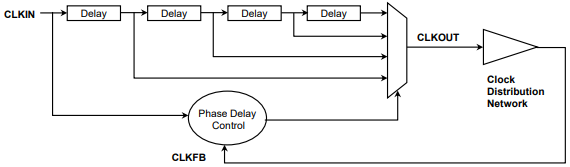
\includegraphics[width=\columnwidth]{img_6.png}
\end{figure}
\subsection{Routage}
BUFIO2 permet de router les signaux d'horloge d'entrée sur des lignes dédiées pour atteindre des horloges I/O, des PLL/DCM ou des buffers BUFG.\\
Les CMT sont situés dans la colonne centrale du FPGA
\subsection{Mémoires}
\begin{itemize}
\item SDR : Lecture/écriture uniquement sur le flanc montant/descendant
\item DDR : Lecture/écriture sur les flancs montants et descendants
\end{itemize}
\subsection{DLL}
\begin{itemize}
\item \SI{5}{\mega\hertz} à \SI{250}{\mega\hertz}
\item De-skew
\item Correction du rapport cyclique
\item Décalage de phase
\end{itemize}
\subsection{Synchronisation}
Utilisation d'un 2-FF (dual flip-flip synchroniser)




\end{document}